\clearpage
\begin{longtable} { | c | p{12cm} | c | } 
\hline
	ID 	&	Issues	&		 Es. hours \\\hline
	56	&	Handle no child from Launcher	&	8 hour	\\\hline
\caption{Issue ID 56}
\label{tab:spr4_nochildfromlauncher}
\end{longtable}

At the end of sprint 3, it was decided by GIRAF to change the way logging in to the Launcher works. It would now be possible to enter the launcher without having a \ct{childId} set, and Sekvens needs a childId to run. This means we had to check whether or not the \ct{childId} was equals to 0, and force the user to select a child if none is chosen. When Sekvens is opened without a child, a \ct{GProfileSelector} pops up with all the children connected to the guardian. This behavior can be seen in \ref{fig:profileselector}.

\begin{figure}[H]
	\centering
	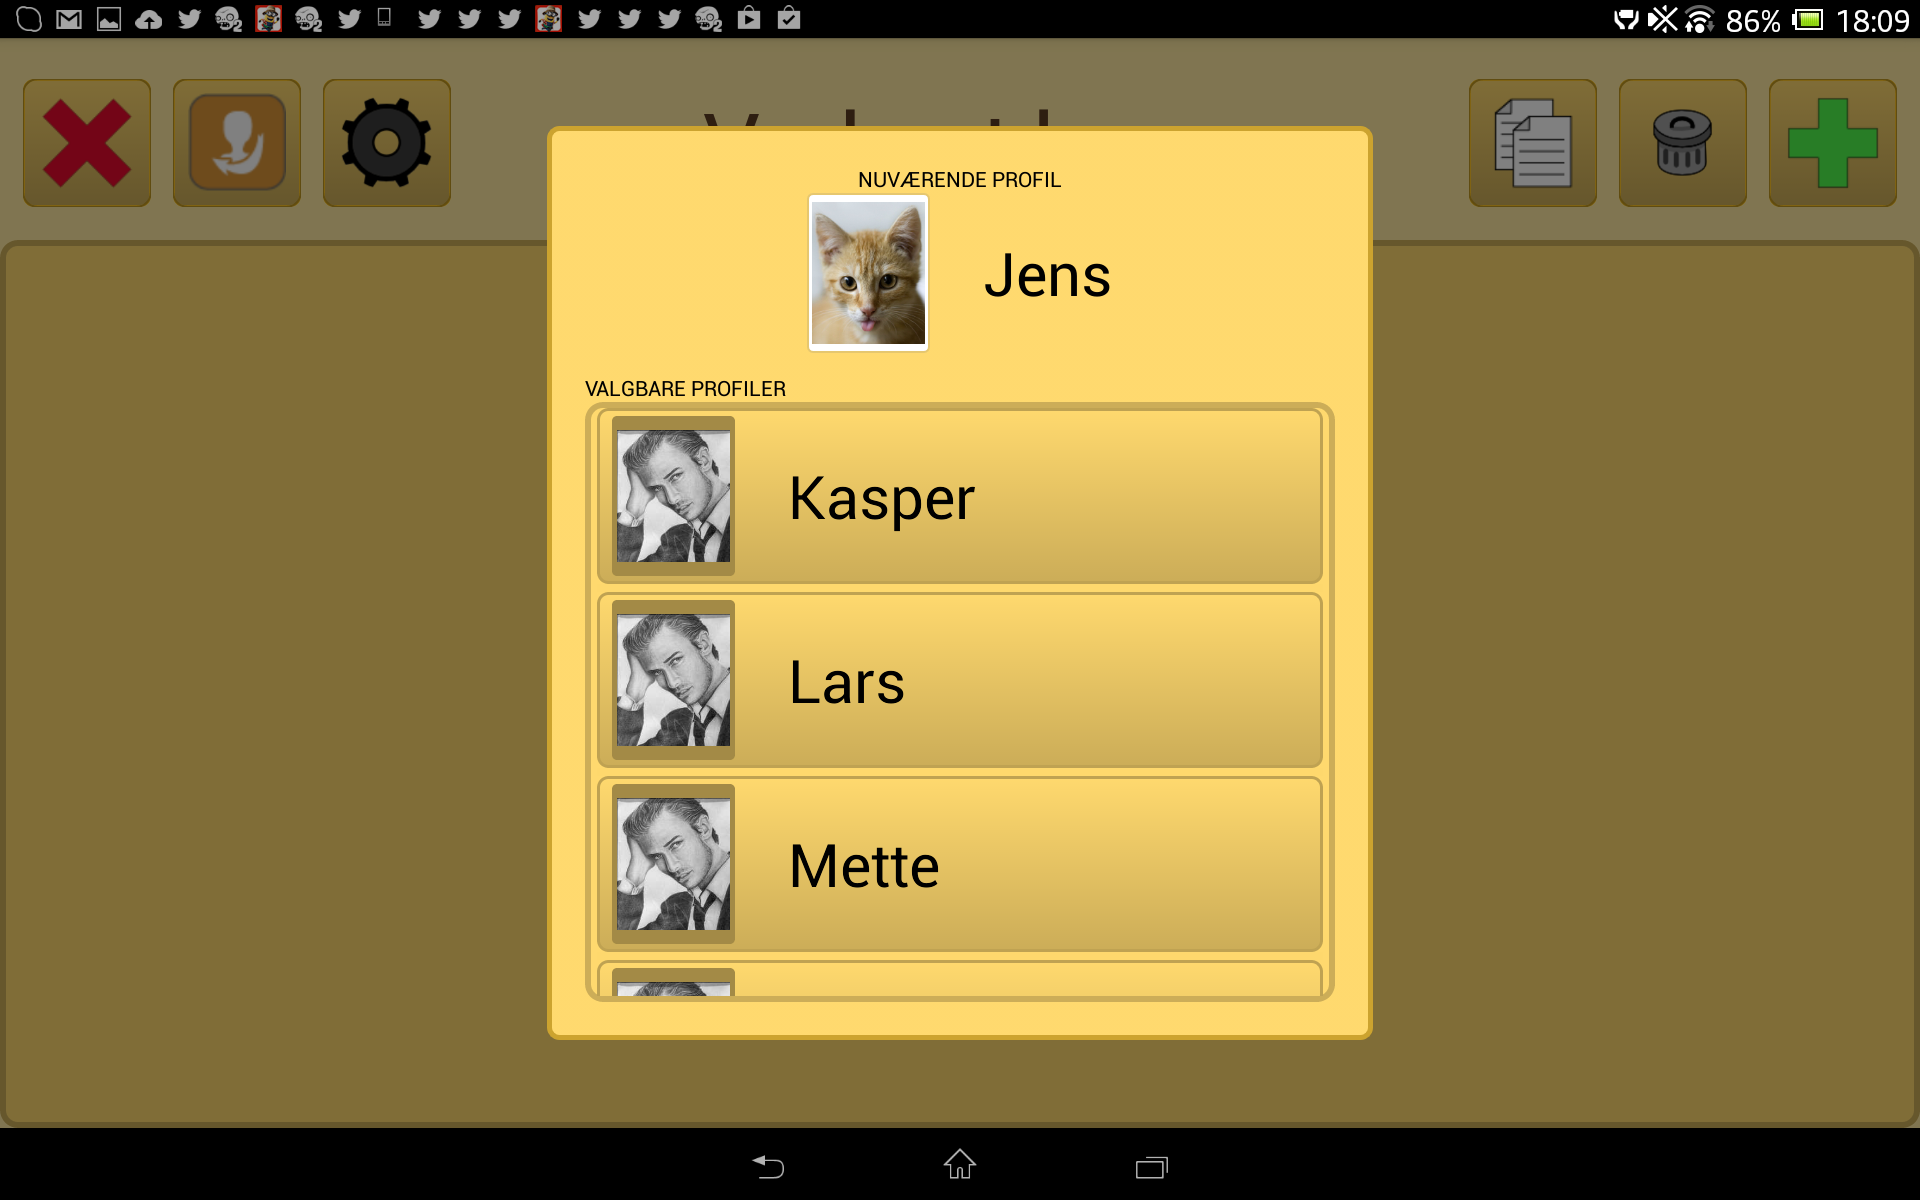
\includegraphics[width=\textwidth]{Pics/Sprint4/profileselector.png}
	\caption{Guardian must pick a child to continue}
	\label{fig:profileselector}
\end{figure}